%%%%%%%%%%%%%%%%%%%%%%%%%%%%%%%%%%%%%%%%%%%%%%
%%%%%%%%%%%%%%%%%%%%%%%%%%%%%%%%%%%%%%%%%%%%%%
%%			     Anexo B     			    %%
%%%%%%%%%%%%%%%%%%%%%%%%%%%%%%%%%%%%%%%%%%%%%%
%%%%%%%%%%%%%%%%%%%%%%%%%%%%%%%%%%%%%%%%%%%%%%
\chapter{Pruebas cliente/servidor con netcat} \label{anexoB}
\newpage

Existe una herramienta de Linux cuya función es crear un cliente y un servidor de una conexión UCP y TCP local llamada ``netcat''. Si el sistema no dispone de ella, se puede instalar fácilmente introduciendo la siguiente orden en el terminal: \\

\begin{bashcode}
$ sudo apt-get install netcat
\end{bashcode}

Para conocer su funcionamiento una vez instalada, se procede a crear un servidor y un cliente locales. Debido a que la comunicación Raspberry Pi Zero - Arduino es TCP, en este ejemplo se opta por dicho modo.
En primer lugar, se abren dos ventanas del terminal, cada una para un rol distinto. En una de ellas, se crea el servidor TCP. Es necesario habilitar el modo ``escucha'' del servidor con la opción ``-l'' y el puerto local con ``-p'' seguido del número del puerto: \\

\begin{bashcode}
$ nc -l -p 25
\end{bashcode}

Si el terminal informa que el puerto no está disponible, es mejor mirar previamente los puertos locales TCP ocupados: \\

\begin{bashcode}
$ nc -vz 127.0.0.1 1-8080
\end{bashcode}

En el código anterior, ``127.0.0.1'' es la dirección IP local y ``1-8080'' indica que se revise el estado desde el puerto 1 hasta el 8080.

Una vez creado el servidor, se puede establecer el servidor:\\

\begin{bashcode}
$ nc 127.0.01 25
\end{bashcode}

A continuación, en la imagen inferior, se observa el resultado:\\

    \begin{figure}
    \centering
    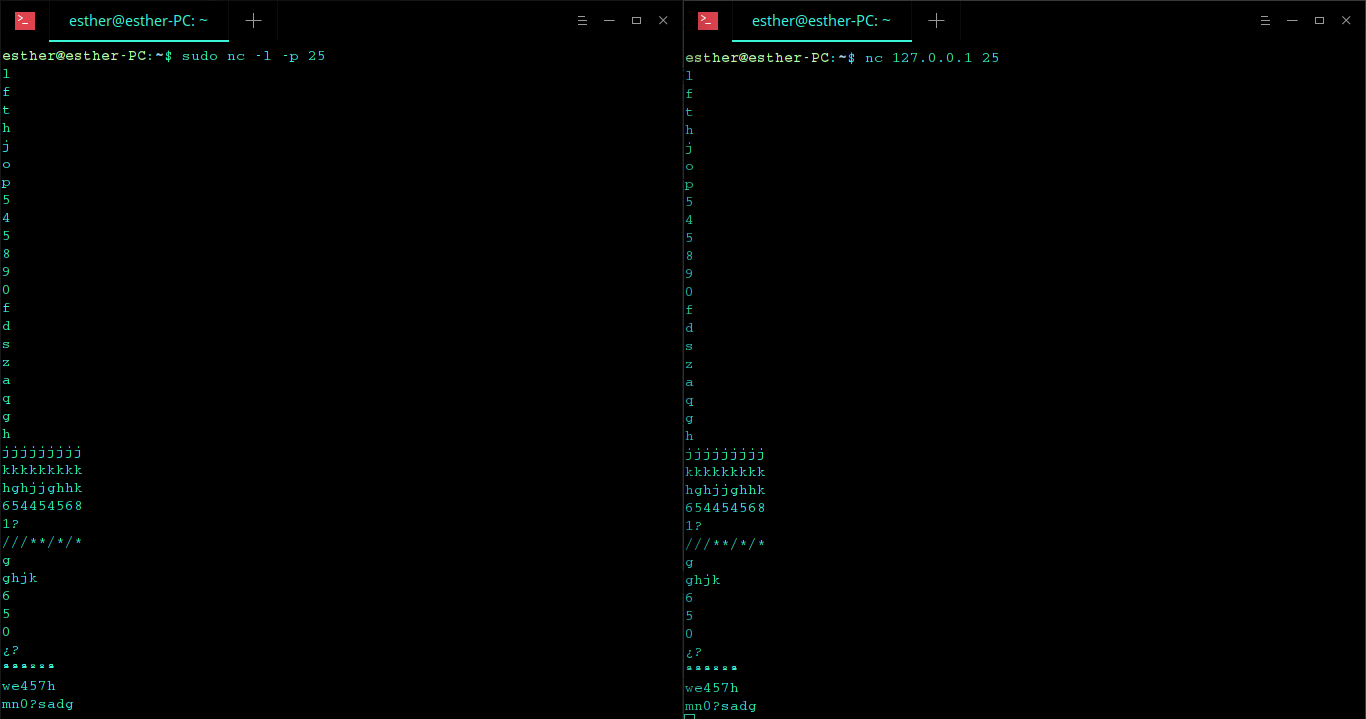
\includegraphics[scale = 0.3]{anexo_b/figuras_dir/csnetcat.jpg}
    \caption{Conexión entre el servidor y cliente netcat}
    %\label{fig:figura4}
    \end{figure}
    
Como se observa en la imagen, todos los datos introducidos en el terminal del cliente, llegan al terminal del servidor y viceversa.

La utilidad que tiene ``netcat'' en el proyecto es la de comprobar el funcionamiento del programa ``Cliente.c''. En la sección 3.3, se comenta que este programa constituye el cliente de la comunicación TCP entre Raspberry Pi Zero y Arduino Leonardo. Para saber si desempeña correctamente esta función, se puede crear un servidor con ``netcat'' que se comunique con el cliente de Raspberry. ``Cliente.c'' se ha elaborado modificando el programa cliente TCP del apartado de ``comunicaciones en red'' del libro del taller \citep{franciscoTCP}. Este programa recoge todo aquello introducido en el terminal del cliente mediante la función ``fgets()'' que lee el descriptor de la entrada estándar (teclado). Evidentemente, la comprobación se puede realizar con el programa cliente original pero la forma más directa de comprobarlo es mediante el programa cliente del taller.

\begin{listing}
\begin{minted}[bgcolor=bg,
               frame=lines,
               framesep=2mm,
               linenos]
               {C}
#include <stdio.h>
#include <stdlib.h>
#include <unistd.h>
#include <assert.h>
#include <string.h>
#include <netdb.h>
#include <arpa/inet.h>

static int tcp_client_socket(const char* host, const char* service);
int main() {
	int fd = tcp_client_socket("127.0.0.1", "25");
	for(;;) {
		char buf[1024];
		fgets(buf, sizeof(buf), stdin);
		int n = write(fd, buf, strlen(buf));
		assert(n >= 0);
		if (n == 0) break;
	}
	close(fd);
	return 0;
}

static struct sockaddr_in ip_address(const char* host,
				const char* service,
				const char* proto);
static int tcp_client_socket(const char* host, const char* service)
{
	struct sockaddr_in sin = ip_address(host, service, "tcp");
	struct protoent* pe = getprotobyname("tcp");
	assert(pe != NULL);
	int fd = socket(PF_INET, SOCK_STREAM, pe->p_proto);
	assert (fd >= 0);
	assert (connect(fd, (struct sockaddr*)&sin, sizeof(sin)) >= 0);
	return fd;
}


static struct sockaddr_in ip_address(const char* host,
				const char* service,
				const char* proto)
{
	struct sockaddr_in sin;
	memset(&sin, 0, sizeof(sin));
	sin.sin_family = AF_INET;
	struct hostent* he = gethostbyname(host);
	if (he != NULL)
	memcpy(&sin.sin_addr, he->h_addr_list[0], he->h_length);
	else
	sin.sin_addr.s_addr = inet_addr(host);
	struct servent* se = getservbyname(service, proto);
	sin.sin_port = (se != NULL? se->s_port : htons(atoi(service)));
	return sin;
}



\end{minted}
\caption{Programa cliente del libro del taller de Raspberry Pi}
\label{Listing}
\end{listing}


Como se observa, el programa se ha modificado para conectarse a la IP local y al puerto 25. Con ello, se procede a establecer la comunicación. El resultado se muestra en la figura \ref{fig:sernet}:

    \begin{figure}
    \centering
    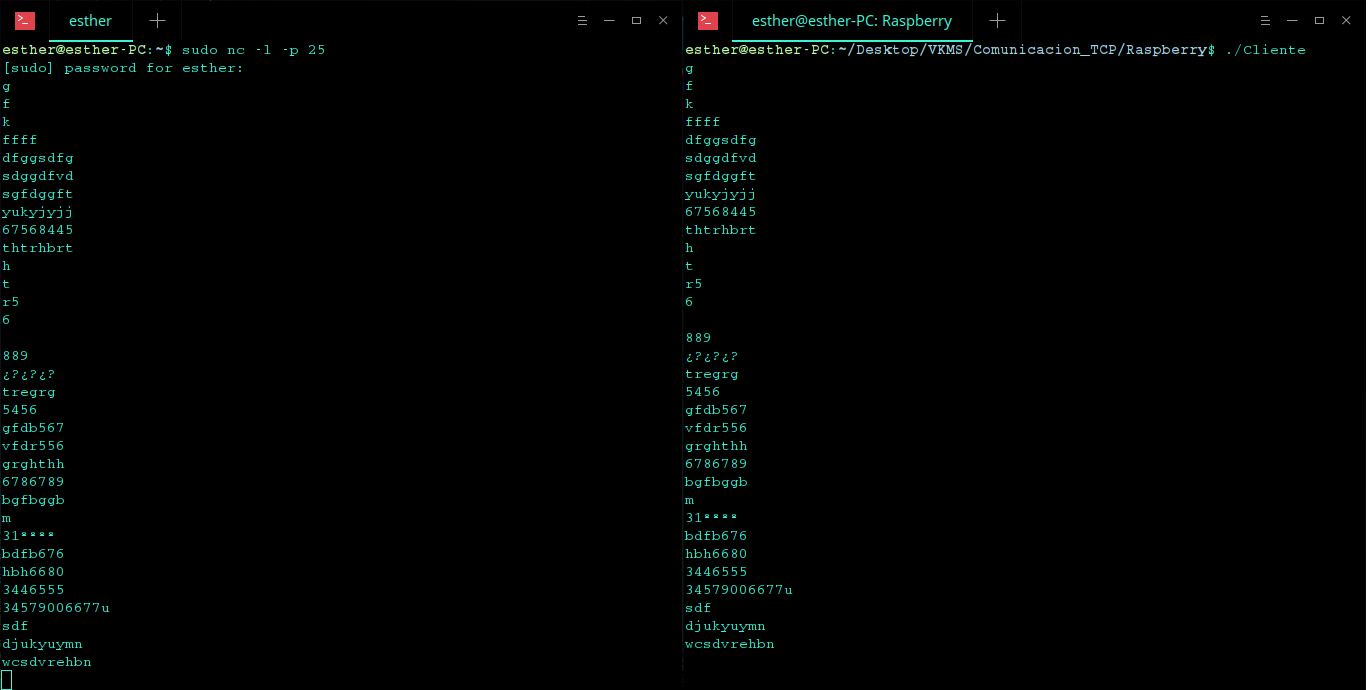
\includegraphics[scale = 0.3]{anexo_b/figuras_dir/sernet.jpg}
    \caption{Conexión entre el servidor netcat y el cliente Raspberry Pi}
    \label{fig:sernet}
    \end{figure}








